\documentclass{article}
\usepackage{amsmath}
\usepackage{braket}
\usepackage{amssymb}
\usepackage{hyperref}
\usepackage{booktabs}
\usepackage{graphicx}
\newcommand{\bfit}[1]{\textit{\textbf{#1}}}
\begin{document}
\textbf{\Large Chapter 9\\
Spin Qubit-Rabi Oscialltion}\\\\\\
\textbf{\large 9.1 Introduction}\\\\
In the previous chapter, we implemented a physical system to perform a phase-shift gate
of arbitrary phase for an electron spin qubit. It is constructed by placing the electron
spin qubit in a constant external magnetic field in the vertical direction, $\vec{B}=-B_0\hat{z}$
with $B_0>0$. This is a field pointing downward in the real 3D space. It causes
Larmor precession of the qubit on the Bloch sphere rotating clockwise looking from the top.
In this chapter, we will further apply a small oscillating magnetic field in the 
$\hat{x}$ direction to enable the rotation of the qubit about the $y-axis$. This is called 
Rabi oscillation. With this tool, we will be able to rotate a spin qubit from and to 
any point on the Bloch sphere and thus implement an arbitrary 1-qubit gate.

More inportantly, in this process, we will clarify some mathematical skills and
also introduce the concept of rotating frame and rotating wave approximation.\\\\
\bfit{\large 9.1.1 Learning Outcomes}\\\\
Understand the role of the small sociallating magnetic field; be able to describe
how a state moves on the Bloch sphere during Rabi oscillation; appreciate the power and
limitation of the perturbation method; understand rotation wave approximation and the 
meaning of rotating frame.\\\\
\bfit{\large 9.1.2 Teaching Videos}\\\\
$\bullet$ Search for Ch9 in this playlist

- \url{https://tinyurl.com/3yhze3jn}\\\\
$\bullet$ Other Videos

- \url{https://youtu.be/5u-vr6-awNc}

- \url{https://youtu.be/XoHVvXTDyQU}

- \url{https://youtu.be/ImFNULXkR_I}

- \url{https://youtu.be/bEEO0bmi-M4}

- \url{https://youtu.be/ndXeb6YcPy0}

- \url{https://youtu.be/GLTHGGPKGuo}
\\\\
\textbf{\large 9.2 Spin Angular Momentum Operator}\\\\
In the previous chapter, we constructed the \textit{Hamiltonian} under a constant vertical
magnetic field using the eigenenergies found in the experiment (Eq.(8.3)). When we have an
oscillating magnetic field. It is difficult to use the same approach because the direction of the 
effective magnetic field is not canstant. Therefore, we need a more formal approach and 
introduce the concept of \textbf{spin angular momentum operator}.

As mentioned in Chap.7, the spin magnetic moment of an electron, $\hat{\mu_e}$, is a result
of spin angular momentum, $\vec{S}$ (Eq.(7.9)). The interaction Hamiltonian between
the magnetic moment and the external magnetic field, $\vec{B}$, is given in Eq.(8.1) and 
repeated here for convenience,
\begin{align*}\label{eq 9.1}
    H&=-\vec{B}\cdot\vec{\mu},\\
    &=-\vec{B}\cdot\gamma\vec{S}.\tag{9.1}
\end{align*} 

When deducing the eigenenergies, we implicitly set $\vec{S}=\frac{\hbar}{2}\hat{z}$ and Eq.(9.1) is
just an inner product of two \textit{real space 3D vectors},$\vec{B}$ and $\vec{S}$.
We then use the eigenenergies to construct Eq.(8.3). That means \textit{we have treated the spin angular
momentum as a vector}. In order to handle a more general case, in which \textit{the net magnetic
field direction is a variable}, we need to use another formalism by treating
the spin angular momentum as an operator. We will not study the formalism and we will 
take it for granted. The mathematics just works out and agrees with experiments.
We define the spin angular momentum operator as 
\begin{align*}\label{eq 9.2}
    \vec{S}&=\frac{\hbar}{2}\boldsymbol{\sigma},\\
    &=\frac{\hbar}{2}(\boldsymbol{\sigma_x}\hat{x}+\boldsymbol{\sigma_y}\hat{y}\boldsymbol{\sigma_z}\hat{z}),\\
    &=\frac{\hbar}{2}\left[\begin{pmatrix}
        0\ 1\\ 1\ 0
    \end{pmatrix}\hat{x}+
    \begin{pmatrix}
        0&-i\\i&0
    \end{pmatrix}\hat{y}+
    \begin{pmatrix}
        1&0\\0&-1
    \end{pmatrix}\hat{z}\right],\\
    &=\frac{\hbar}{2}\begin{pmatrix}
        \hat{z}&\hat{x}-i\hat{y}\\
        \hat{x}+i\hat{y}&-\hat{z}
    \end{pmatrix},\tag{9.2}
\end{align*}
where the Pauli vector, $\vec{\boldsymbol{\sigma}}$, is used (see Chapter 7 of [1] and Eq. (6.4)).
Note the $\vec{S}$ still a vector in the linear algebara sense (it obeys the definition of vector in a vector space)
but it is also an operator now.

Therefore, Eq. (\ref{eq 9.1}) becomes
\begin{equation}\label{eq 9.3}
    \boldsymbol{H}=-\vec{B}\cdot\gamma\vec{S}.\tag{9.3}
\end{equation}

We take the definition of spin angular momentum operator for granted but we can 
check if this makes sense.\\\\
\textbf{Example 9.1} Find the expectation calue of $\vec{S}$ in state $\ket{0}$.

We know that $\ket{0}$ is $\ket{\uparrow}$ (Fig.8.1) and it has a spin value of $\frac{1}{2}$ 
and should be in the $+\hat{z}$ direction. Based on Eq. (7.7), the spin angular momentum is $\frac{\hbar}{2}\hat{z}$.

Let us find the expectation value of $\vec{S}$ in state $\ket{0}$, which is
\begin{align*}\label{eq 9.4}
    \braket{0|\: \vec{\boldsymbol{S}} \:|0}&=\begin{pmatrix}
        1\ 0
    \end{pmatrix}\frac{\hbar}{2}
    \begin{pmatrix}
        \hat{z}&\hat{x}-i\hat{y}\\
        \hat{x}+i\hat{y}&-\hat{z}
    \end{pmatrix}
    \begin{pmatrix}
        1\\0
    \end{pmatrix},\\
    &=\frac{\hbar}{2}\begin{pmatrix}
        1\ 0
    \end{pmatrix}
    \begin{pmatrix}
        \hat{z}\\\hat{x}+i\hat{y}
    \end{pmatrix},\\
    &=\frac{\hbar}{2}\hat{z}.\tag{9.4}
\end{align*}

This is the same as what we expected with the correct magnitude and also direction.\\\\
\textbf{\large 9.3 Rabi Oscialltion}\\\\
\bfit{\large 9.3.1 Experimental Setup and Hamiltonian}\\\\
The setup for \textbf{Rabi Oscillation} is shown in Fig. 9.1. It is the same as Fig. 8.1
except that a small osciallting magnetic field is applied along the $\hat{x}$ direction, with 
$B_1\ll B_0$. The oscillating magnetic field socillates at an angular frequency of $\omega_1$.
To understand how the qubit will evolve, we need to first find the \textit{Hamiltonian} using
Eq. (\ref{eq 9.3}).

Firstly, the total magnetic field, $\vec{B}$, at any time, is given by
\begin{equation}\label{eq 9.5}
    \vec{B}=B_1\cos(\omega_1t)\hat{x}-B_0\hat{z}.\tag{9.5}
\end{equation}
\\\\
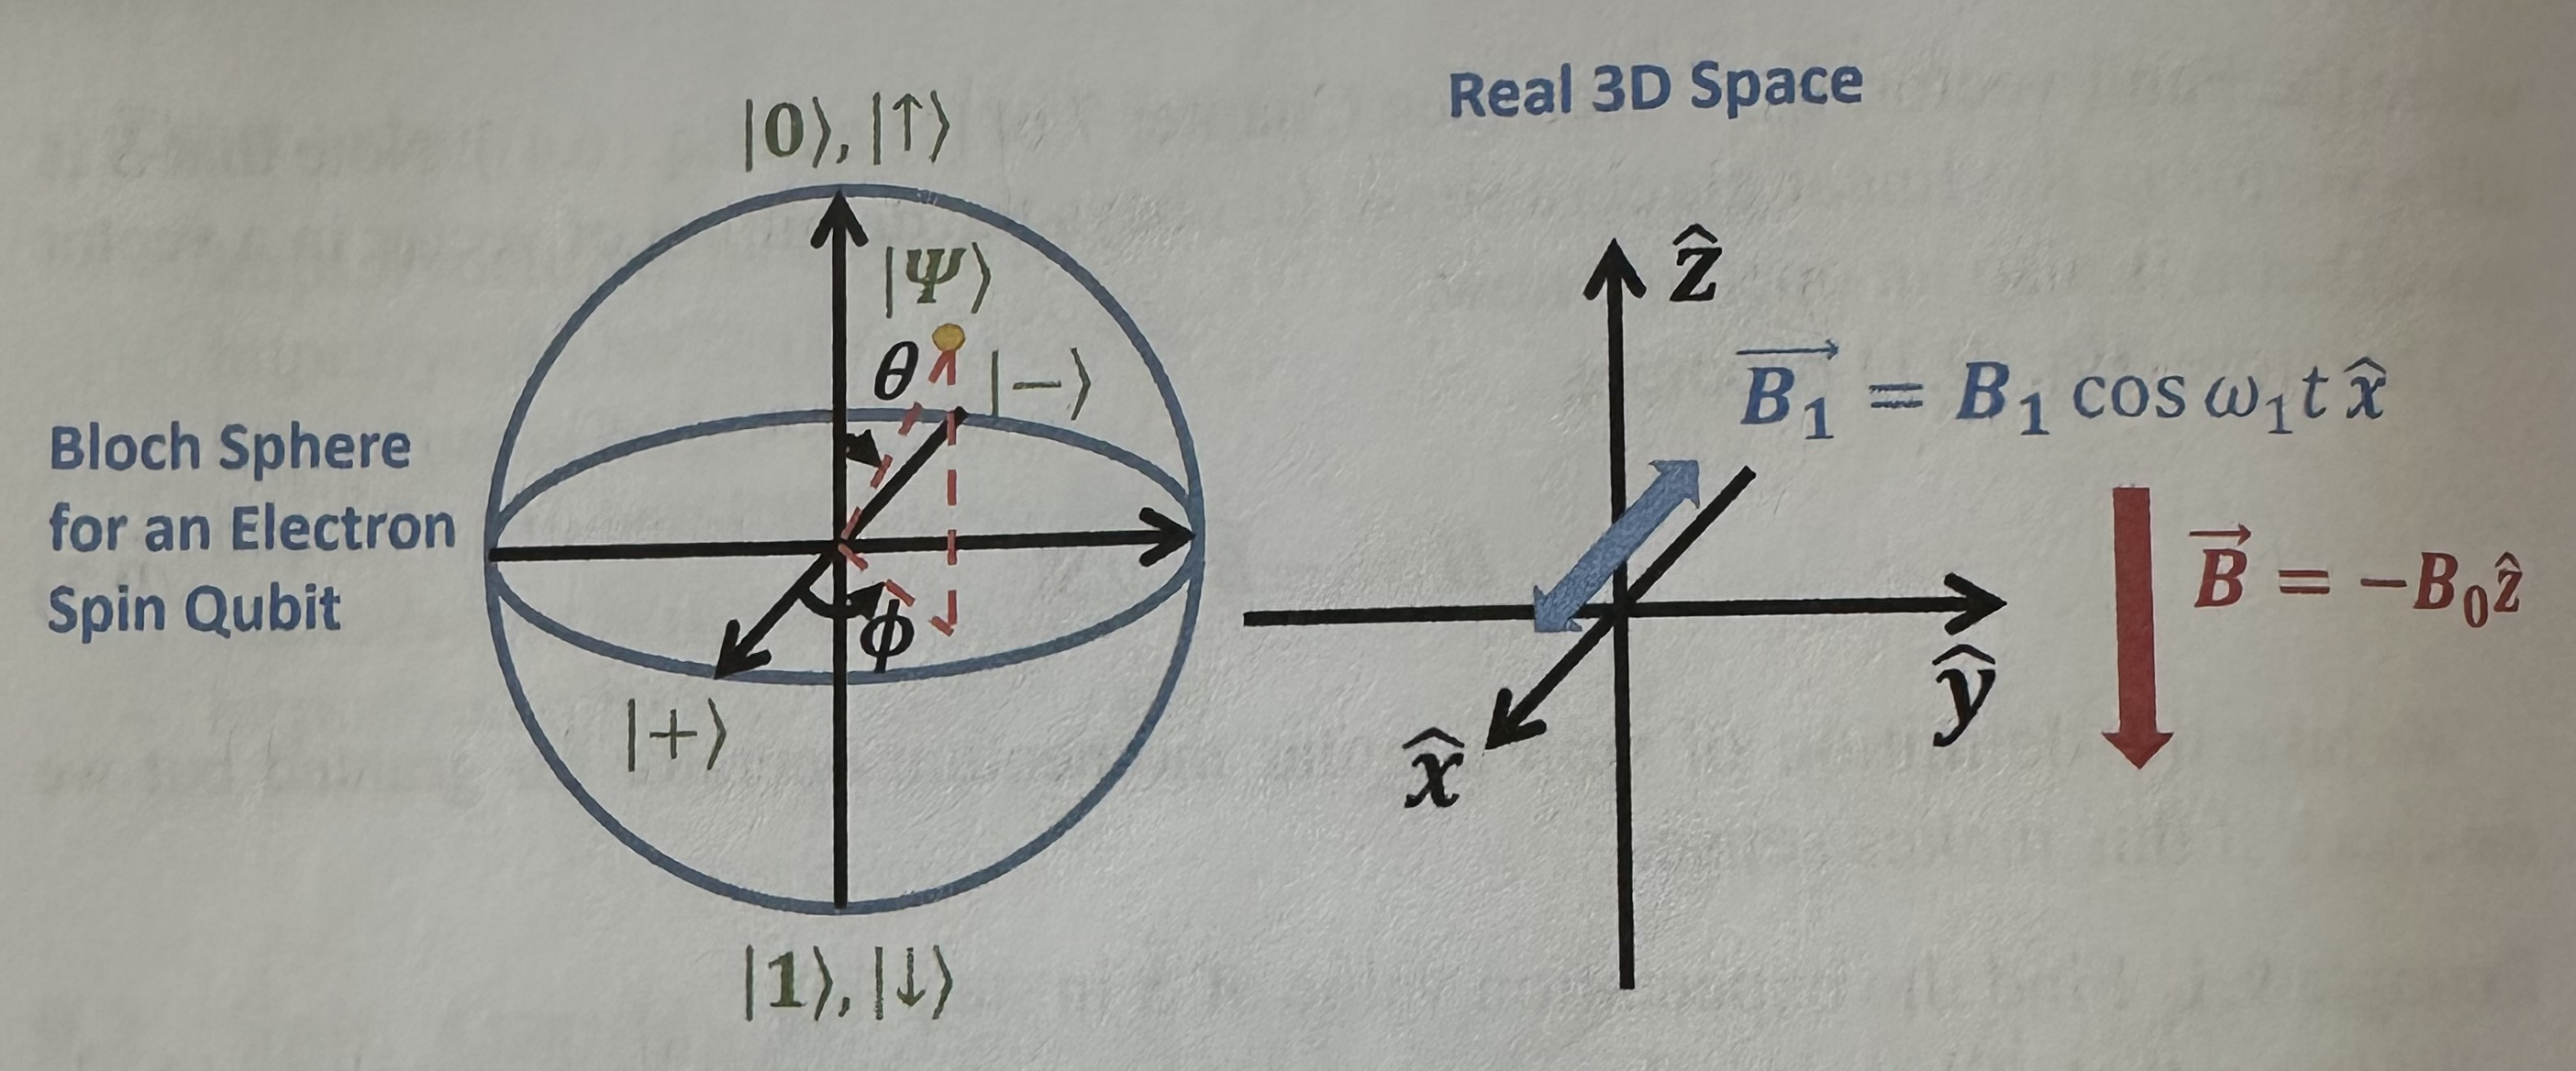
\includegraphics[scale=0.5]{Fig.9.1.jpeg}\\
\textbf{Fig. 9.1} The Bloch sphere representation of an electron spin qubit (left) and the real 3D space 
coordinate system in which the direction of the external constant and osillating magnetic fields
is shown\\

Therefore, the Hamiltonian is given by Eq.(\ref{eq 9.3}):
\begin{align*}\label{eq 9.6}
    \boldsymbol{H}&=-\vec{B}\cdot\gamma\vec{\boldsymbol{S}},\\
    &\approx\left(\frac{e}{m}\vec{\boldsymbol{S}}\right)\cdot\vec{B},\\
    &=\frac{e\hbar}{2m}(\boldsymbol{\sigma_x}\hat{x}+\boldsymbol{\sigma_y}\hat{y}+\boldsymbol{\sigma_z}\hat{z})\cdot
    (B_x\hat{x}+B_y\hat{y}+B_z\hat{z}),\\
    &=\frac{e\hbar}{2m}(\boldsymbol{\sigma_x}\ \boldsymbol{\sigma_y}\ \boldsymbol{\sigma_z})\begin{pmatrix}
        B_1\cos(\omega_1t)\\
        0\\
        -B_0
    \end{pmatrix},\\
    &=\frac{e\hbar}{2m}B_1\cos(\omega_1t)\boldsymbol{\sigma_x}-\frac{e\hbar}{2m}B_0\boldsymbol{\sigma_z},\\
    &=\frac{e\hbar}{2m}B_1\cos(\omega_1t)\boldsymbol{\sigma_x}-\frac{\hbar\omega_L}{2}B_0\boldsymbol{\sigma_z},\\
    &=\boldsymbol{H_1}+\boldsymbol{H_0}. \tag{9.6}
\end{align*}
where in line 2, we used the approximation of $g\approx-2$ (see Eqs.(7.8) and(7.9)). It should also
be noted that $e=1.6\times10^{-19}C<0$. In line 3, we used Eq. (\ref{eq 9.2}. In line 4
Eq. (\ref{eq 9.5}) was used. In line 6, we used the deifinition of Larmor frequency in Eq. (8.11).

The Hmailtonian is separated into two parts, namely, $\boldsymbol{H_0}=-\frac{e\hbar}{2m}B_0\boldsymbol{\sigma_z}$
and $\boldsymbol{H_1}=\frac{e\hbar}{2m}B_1\cdot(\omega_1t)\boldsymbol{\sigma_x}\cdot\boldsymbol{H_0}$ is the same
as Eq. (8.4), which is the Hamiltonian due to the interaction of the vertical constant magnetic
field and the spin magnetic moment. We know this causes the spin to precess about the vertical axis on the
Bloch sphere. $\boldsymbol{H_1}$ is new and it is due to the transverse oscillating magnetic field
and is a function of $B_1$ and $\omega_1$.\\\\
\bfit{\large 9.3.2 Setup of the Schr\"{o}dinger Equation}\\\\
The Schr\"{o}dinger equation corresponding to this system is given by
\begin{equation}\label{eq 9.7}
    i\hbar\frac{\partial\ket{\psi}}{\partial t}=(\boldsymbol{H_0}+\boldsymbol{H_1})\ket{\psi},\tag{9.7}\\
\end{equation}
with $\boldsymbol{H_0}$ and $\boldsymbol{H_1}$ defined in Eq. (\ref{eq 9.6}). It is not tricial to solve this equation.
However, as mentioned at the beginning of this section, we assume $B_1\ll B_0$.
Then the oscillating magnetic field in the $\hat{x}$ direction can be treated as a \textbf{perturbation}
of the original system in Fig. 8.1 (i.e., only with a constant vertical magnetic field).

It is known that if a perturbation is added to a system, the state of the new system,
$\ket{\Psi_{perturbed}}$, is a linear combination of the eigenstates ($\ket{0}, \ket{1},\cdots$) of
unperturbed system weighted by the complex exponential of the scaled eigenenrgies ($-E_0t/\hbar, -E_1t/\hbar,\cdots$).
Interested readers can refer to time-dependent perturbation in any quantum mechanics textbook such as
[2] for more details. That is,
\begin{equation}\label{eq 9.8}
    \ket{\Psi_{perturbed}}=c_0e^{-iE_0t/\hbar}\ket{0}+c_1e^{-iE_1t\hbar}\ket{1}+\cdots,\tag{9.8}
\end{equation}
where $c_0, c_1,\cdots$ are complex coefficients and can be time-dependent.

In our case, the \textit{unperturbed system} (i.e., without the oscillating field) has two
eigenstates $\ket{0}$ and $\ket{1}$ with eigenenergies $-|\vec{B}||\vec{\mu}|=-\hbar\omega_L/2$ and
$|\vec{B}||\vec{\mu}|=\hbar\omega_L/2$, respectively (see the discussion in Sect. 8.2 and
Eqs. (8.13) and (8.14)). Therefore, the state of the new system with the perturbing osciallting
magnetic field can be written as
\begin{align*}\label{eq 9.9}
    \ket{\Psi_{perturbed}}&=c_0e^{-i\frac{E_0t}{\hbar}}\ket{0}+
    c_1e^{-i\frac{E_1t}{\hbar}}\ket{1},\\
    &=c_0e^{-i\frac{-\hbar\omega_Lt}{2\hbar}}\ket{0}+c_1e^{-i\frac{-\hbar\omega_Lt}{2\hbar}}\ket{1},\\
    &=c_0e^{i\frac{\omega_L}{2}t}\ket{0}+c_1e^{-i\frac{\omega_L}{2}t}\ket{1}.\tag{9.9}\\
\end{align*}

Note that $\ket{\Psi_perturbed}$ is just the $\ket{\Psi}$ in Eq.{\ref{eq 9.7}}. We will now only
use $\ket{\Psi}$. 

We should also remember that the wavefunction needs to be normalized.
Therefore,
\begin{align*}\label{eq 9.10}
    |c_0|^2+|c_1|^2&=1,\\
    |c_0(t)|^2+|c_1(t)|^2&=1,\tag{9.10}
\end{align*}
where we emphasized that $c_0$ and $c_1$ can be time-dependent in the second line.
\\\\
\bfit{\large 9.3.3 Solving the Schr\"{o}dinger Equation}\\\\
Now, we will solve Eq. (\ref{eq 9.7}) by substituting Eq. (\ref{eq 9.9}) into it.
This is lengthy derivation. If you feel this too long, you may skip and just trust the answer.
If not, I  hope you can follow closely as we will pracgice some very useful skills
in quantum mechanics.

We first perform the substitution.
\begin{align*}\label{eq 9.11}
    i\hbar\frac{\partial\ket{\psi}}{\partial t}&=(\boldsymbol{H_0}+\boldsymbol{H_1})\ket{\psi},\\
    i\hbar\frac{\partial(c_0e^{i\frac{\omega_L}{2}t}\ket{0}+c_1e^{-i\frac{\omega_L}{2}t}\ket{1})}{\partial t}
    &=(\boldsymbol{H_0}+\boldsymbol{H_1})(c_0e^{i\frac{\omega_L}{2}t})\ket{0}\\
    &+c_1e^{-i\frac{\omega_L}{2}t}\ket{1}).\tag{9.11}
\end{align*}

Let us first simplify the \textit{left-hand side}.
\begin{align*}\label{eq 9.12}
    i\hbar\frac{\partial \ket{\psi}}{\partial t}&=i\hbar\bigg( \dot{c_0}e^{i\frac{\omega_L}{2}t}\ket{0}+c_0(i\frac{\omega_L}{2})e^{i\frac{\omega_L}{2}t}\ket{0}\\
    &+\dot{c_1}e^{-i\frac{\omega_L}{2}t}\ket{1}+c_1(-i\frac{\omega_L}{2})e^{-i\frac{\omega_L}{2}t}\ket{1} \bigg),   \tag{9.12}
\end{align*}
where we use the chain ruel in derivatices. We also use the common notation of time derivatice,
$\dot{c}=\frac{dc}{dt}$. We will now apply an inner product with $\ket{0}$ to Eq. (\ref{eq 9.12}).
This is equivalent to applying $\bra{0}$ from the left,
\begin{align*}\label{eq 9.13}
    &\bra{0}i\hbar\bigg( \dot{c_0}e^{i\frac{\omega_L}{2}t}\ket{0}+c_0(i\frac{\omega_L}{2})e^{i\frac{\omega_L}{2}t}\ket{0}\\
    &+\dot{c_1}e^{-i\frac{\omega_L}{2}t}\ket{1}+c_1(-i\frac{\omega_L}{2}e^{-i\frac{\omega_L}{2}t})\ket{1}\bigg),\\
    =&i\hbar\bigg(\dot{c_0}e^{i\frac{\omega_L}{2}t}\braket{0|0}+c_0(i\frac{\omega_L}{2})e^{i\frac{\omega_L}{2}t}\braket{0|0}\\
    &+dot{c_1}e^{-i\frac{\omega_L}{2}t}\braket{0|1}+c_1(-i\frac{\omega_L}{2}e^{-i\frac{\omega_L}{2}t})\braket{0|1}\bigg),\\
    =&i\hbar\bigg(\dot{c_0}e^{i\frac{\omega_L}{2}t}+c_0(i\frac{\omega_L}{2}t)e^{i\frac{\omega_L}{2}t}\bigg).\tag{9.13}
\end{align*}
where we have used the fact that $\ket{0}$ and $\ket{1}$ are \textit{orthonormal} in the last step.
Therefore, $\braket{0|0}=1$ and $\braket{0|1}=0$.

Now, we will simplify the right-hand side and apply $\bra{0}$ from the left. From Eq. (\ref{eq 9.11}),
\begin{align*}\label{eq 9.14}
    &\bra{0}(\boldsymbol{H_0}+\boldsymbol{H_1}(c_0e^{i\frac{\omega_L}{2}t}\ket{0}+c_1e^{-i\frac{\omega_L}{2}t})\ket{1}),\\
    =&\bra{0}\bigg(\boldsymbol{H_0}c_0e^{i\frac{\omega_L}{2}t}\ket{0}+\boldsymbol{H_1}c_1e^{-i\frac{\omega_L}{2}t})\ket{1}\\
    &+\boldsymbol{H_1}c_0e^{i\frac{\omega_L}{2}t}\ket{0}+\boldsymbol{H_1}c_1e^{-i\frac{\omega_L}{2}t}\ket{1}\bigg),\\
    =&c_0e^{i\frac{\omega_L}{2}t}\braket{0|\boldsymbol{H_0}|0}+c_1e^{-i\frac{\omega_L}{2}t}\braket{0|\boldsymbol{H_0}|1}\\
    &+c_0e^{i\frac{\omega_L}{2}t}\braket{0|\boldsymbol{H_1}|0}+c_1e^{-i\frac{\omega_L}{2}t}\braket{0|\boldsymbol{H_1}|1} \tag{9.14}
\end{align*}

Now, we need to evaluate $\braket{0|\boldsymbol{H_0}|0}, \braket{0|\boldsymbol{H_1}|1}, \braket{0|\boldsymbol{H_1}|0}$,
 and $\braket{0|\boldsymbol{H_1}|1}$. Firstly, since $\ket{0}$ and $\ket{1}$ are the eigenstates of the unperturbed system, 
 $\boldsymbol{H_0}$, we have,
\begin{align*}\label{eq 9.15}
    \braket{0|\boldsymbol{H_0}|0}&=\bra{0}(-\hbar\omega_L/2)\ket{0}),\\
    &=-\hbar\omega_L/2\braket{0|0},\\
    &=-\hbar\omega_L/2,\tag{9.15}
\end{align*}
and
\begin{align*}\label{eq 9.16}
    \braket{0|\boldsymbol{H_0}|1}&=\bra{0}(-\hbar\omega_L/2)\ket{1}),\\
    &=-\hbar\omega_L/2\braket{0|1},\\
    &=0,\tag{9.16}
\end{align*}
where we used the fact that applying the Hamiltonian to its eigenvector results in the eigenvector
scaled by the corresponding eigenvalue. We could have also used the matrix form
of $\boldsymbol{H_0}=-\frac{\hbar\omega_L}{2}\boldsymbol{\sigma_z}$ in Eq.(\ref{eq 9.6}) to obtain
the same result.

To evaluate $\braket{0| \boldsymbol{H_1} |0}$ and $\braket{0| \boldsymbol{H_1} |1}$, we will use the definition
of $\boldsymbol{H_1}=\frac{e\hbar}{2m}B_1\cos(\omega_1t)\boldsymbol{\sigma_x}$ in Eq. (\ref{eq 9.6}) and perform
matrix multiplications.
\begin{align*}\label{eq 9.17}
    \braket{0|\boldsymbol{H_1}|0}&=\bra{0}\frac{e\hbar}{2m}B_1\cos(\omega_1t)\boldsymbol{\sigma_x}\ket{0},\\
    &=\frac{e\hbar}{2m}B_1\cos(\omega_1t)\bra{0}\boldsymbol{\sigma_x}\ket{0},\\
    &=\frac{e\hbar}{2m}B_1\cos(\omega_1t)\begin{pmatrix}
        1\ 0
    \end{pmatrix}
    \begin{pmatrix}
        0\ 1\\ 1\ 0
    \end{pmatrix}
    \begin{pmatrix}
        1\\0
    \end{pmatrix},\\
    &=0.\tag{9.17}
\end{align*} 
and
\begin{align*}\label{eq 9.18}
    \braket{0|\boldsymbol{H_1}|1}&=\bra{0}\frac{e\hbar}{2m}B_1\cos(\omega_1t)\boldsymbol{\sigma_x}\ket{1},\\
    &=\frac{e\hbar}{2m}B_1\cos(\omega_1t)\bra{0}\boldsymbol{\sigma_x}\ket{1},\\
    &=\frac{e\hbar}{2m}B_1\cos(\omega_1t)\begin{pmatrix}
        1\ 0
    \end{pmatrix}
    \begin{pmatrix}
        0\ 1\\ 1\ 0
    \end{pmatrix}
    \begin{pmatrix}
        0\\1
    \end{pmatrix},\\
    &=\frac{e\hbar}{2m}B_1\cos(\omega_1t).\tag{9.18}
\end{align*} 

Therefore, only two terms are left in Eq. (\ref{eq 9.14}). By equating it to
Eq. (\ref{eq 9.13}), we have
\begin{align*}\label{eq 9.19}
    &i\hbar\bigg(\dot{c_0}e^{i\frac{\omega_L}{2}t}+c_0(i\frac{\omega_L}{2})e^{i\frac{\omega_L}{2}t}\bigg),\\
    =&c_0e^{i\frac{\omega_L}{2}t}\braket{0|\boldsymbol{H_0}|0}+c_1e^{-i\frac{\omega_L}{2}t}\braket{0|\boldsymbol{H_1}|1},\\
    =&c_0e^{i\frac{\omega_L}{2}t}(-\hbar\omega_L/2)+c_1e^{-i\frac{\omega_L}{2}t}(\frac{e\hbar}{2m}B_1\cos(\omega_1t)).\tag{9.19}
\end{align*}

Equating line 1 and line 3 of Eq. (\ref{eq 9.19}) and recognizing $i\hbar c_0(i\frac{\omega_L}{2})e^{i\frac{\omega_L}{2}t}$ in line 1
and $c_0e^{i\frac{\omega_L}{2}t}(-\hbar\omega_L/2)$ in line 3 are equal and can be canceled, we have
\begin{align*}\label{eq 9.20}
    i\hbar\dot{c_0}e^{i\frac{\omega_L}{2}t}&=c_1e^{-i\frac{\omega_L}{2}t}(\frac{e\hbar}{2m}B_1\cos(\omega_1t)),\\
    i\dot{c_0}&=\frac{e}{2m}B_1\cos(\omega_1t)e^{-i\omega_Lt}c_1.\tag{9.20}
\end{align*}

What we have done so far is to perform an inner product with $\ket{0}$ so that we obtain
the rate of change of $c_0$ as a function of $c_1$. Now if we repeat the same process by applying an inner 
product with $\ket{1}$, we will get an equation relating the rate of change
of $c_1$ as a functino of $c_0$, which is 
\begin{equation}\label{eq 9.21}
    i\dot{c_1}=\frac{e}{2m}B_1\cos(\omega_1t)e^{i\omega_Lt}c_0.\tag{9.21}
\end{equation}

As a reminder,$e>0$. To solve for $c_0$, we can perform one more time differentiation
on Eq. (\ref{eq 9.20}) and substitute Eq. (\ref{eq 9.21}) into it. However, for instructional
purposes, we are not interested in the general solution here. We are intersetd in the case when
$\omega_1=\omega_L$.\\\\
\textbf{\large 9.4 Spin Resonance and Rotating Wave Approximation (RWA)}\\\\
When $\omega_1=\omega_L$, the system is at \textbf{electron spin resonance}. \textit{
    it means that the horizontal oscillating magnetic field oscillates at the same frequency
    as the Larmor frequency
}. By using, $\cos\theta=\frac{e^{i\theta+e^{-i\theta}}}{2}$, Eq. (\ref{eq 9.20}) becomes

\begin{align*} \label{eq 9.22}
    ic_0&=\frac{e}{2m}B_1\cos(\omega_1t)e^{-i\omega_Lt}c_1,\\
    &=\frac{e}{4m}B_1(e^{i\omega_1t}+e^{-i\omega_1t}),\\
    &=\frac{e}{4m}B_1(e^{i(\omega_t-\omega_L)t}+e^{-i(\omega_t-\omega_L)t}c_1,\\
    &=\frac{e}{4m}B_1(e^{i0t}+e^{-iw\omega_Lt})c_1,\\
    &=\frac{e}{4m}B_1(1+e^{-i2\omega_Lt}c_1, \tag{9.22}
\end{align*}
where we have used the fact that $\omega_1=\omega_L$ in line 4 at spin resonance. For the term $e^{-i2\omega_Lt}$ which
is equal to $\cos2\omega_Lt-i\sin2\omega_Lt$, it oscillates very fast compared to the time scale we are interested in. 
Therefore, it can be ignored. This is called the \textbf{rotating wave approximation (RWA)}. We will discuss more about the 
meaning of "fast" and understand it from a more intuitive point of view in the next section. For now, let us accept it and Eq. 
(\ref{eq 9.22}) is simplified to
\begin{equation}\label{eq 9.23}
    i\dot{c_0}=\frac{e}{4m}B_1c_1.\tag{9.23}
\end{equation}

Similarly, by using RWA under spin resonance, Eq. (\ref{eq 9.21}) is simplified to
\begin{equation}\label{eq 9.24}
    i\dot{c_1}=\frac{e}{4m}B_1c_0. \tag{9.24}
\end{equation}

By taking a further time derivative on Eq. (\ref{eq 9.23}) and substituting Eq. (\ref{eq 9.24}) into Eq. (\ref{eq 9.23}),
\begin{align*}\label{eq 9.25}
    \frac{d(i\dot{c_0})}{dt}=i\ddot{c_0}&=\frac{e}{4m}B_1\dot{c_1},\\
    &=\frac{e}{4m}B_1\big(\frac{e}{4mi}B_1c_0\big),\\
    \ddot{c_0}&=-(\frac{B_1e}{4m})^2c_0,\tag{9.25}
\end{align*} 
we obtain a second-order differential euqation for $c_0$. Defining $\omega_R^\prime=\frac{B_1e}{4m}$, the euqation becomes
$\ddot{c_0}=-\omega_R^2c_0$ and the general solution is [3]
\begin{equation}\label{eq 9.26}
    c_0=A\cos\omega_R^\prime t+B\sin\omega_R^\prime t.\tag{9.26}
\end{equation}

To find $c_1$, we will use Eq. (\ref{eq 9.23}) and substitute Eq. (\ref{eq 9.26}) into it,
\begin{align*}\label{eq 9.27}
    c_1&=\frac{i}{\omega_R^\prime}\dot{c_0}=i(-A\sin\omega_R^\prime t+B\cos\omega_R^\prime t),\\
    &=-iA\sin\omega_R^\prime t+iB\cos\omega_R^\prime t.\tag{9.27}
\end{align*}

Note that $c_0$ and $c_1$ are the coefficients (ignoring the phases) of $\ket{0}$ and $\ket{1}$, respectively (Eq.(\ref{eq 9.9})).
Therefore, the square of their magnetitudes represent measurement. Since both of them oscillate at $\omega_R^\prime$, the probabilities of finding
the electron at $\ket{0}$ and $\ket{1}$ thus oscillate with time.\\\\
\textbf{\large 9.5 Rabi Oscillation and Rabi Frequency}\\\\
As shown in Eqs. (\ref{eq 9.26}) and (\ref{eq 9.27}), the movement of the electron state is complex. We now will inspect a special case 
to understand how the spin state moves on the Bloch sphere due to \textbf{Rabi oscillation}.

At time $t=0$, by using Eqs. (\ref{eq 9.26}) and (\ref{eq 9.27}), Eq. (\ref{eq 9.9}) becomes
\begin{align*}\label{eq 9.28}
    \ket{\Psi(t=0)}&=c_0e^{i\frac{\omega_L}{2}0}\ket{0}+c_1e^{-i\frac{\omega_L}{2}0}\ket{1},\\
    &=c_0(t=0)\ket{0}+c_1(t=1)\ket{1},\\
    &=A\ket{0}+iB\ket{1}, \tag{9.28}
\end{align*}
where $A$ and $iB$ are, thus, the coefficients of $\ket{0}$ and $\ket{1}$ at $t=0$, respectively. However, recall that on the Bloch sphere,
the state at $t=0$ is characterized by an initial polar angle ($\theta_0$) and an azimuthal angle ($\phi_0$) (similar to Eq. (8.10)). Therefore,
$A=\cos\frac{\theta_0}{2}\exp\{ -i{\frac{\phi_0}{2}}\}$ and $iB=\sin\frac{\theta_0}{2}\exp\{ i{\frac{\phi_0}{2}}\}$. As a result,
\begin{align*}\label{eq 9.29}
    c_0&=A\cos\omega_R^\prime t+B\sin\omega_R^\prime t,\\
    &=\cos\frac{\theta_0}{2}\exp\{ -i{\frac{\phi_0}{2}}\}\cos\omega_R^\prime t -i\sin{\frac{\theta_0}{2}}\exp\{ i{\frac{\phi_0}{2}}\},\\
    &=e^{-i\frac{\phi_0}{2}}[\cos{\frac{\theta_0}{2}}\cos\omega_R^\prime t-e^{i\frac{\pi}{2}}\sin{\frac{\theta_0}{2}}\sin\omega_R^\prime te^{i\phi_0}],\\
    &=e^{-i\frac{\phi_0}{2}}[\cos{\frac{\theta_0}{2}}\cos\omega_R^\prime t- \sin{\frac{\theta_0}{2}}\sin\omega_R^\prime te^{i(\phi_0+\frac{\pi}{2})}],\tag{9.29}
\end{align*}
where we used the fact that $i=e^{i\frac{\pi}{2}}$ in line 3. Using Eq. (\ref{eq 9.27}), we obtain,
\begin{align*}\label{eq 9.30}
    c_1&=-iA\sin\omega_R^\prime t+iB\cos\omega_R^\prime t,\\
    &= -i\cos{\frac{\theta_0}{2}}\exp\{ -i{\frac{\phi_0}{2}}\}\sin\omega_R^\prime t+\sin{\frac{\theta_0}{2}}\exp\{ i{\frac{\phi_0}{2}}\}cos\omega_R^\prime t,\\
    &=e^{-i\frac{\phi_0}{2}}[\sin{\frac{\theta_0}{2}}\cos\omega_R^\prime t+ \cos{\frac{\theta_0}{2}}\sin\omega_R^\prime te^{-i(\phi_0+\frac{\pi}{2})}],\tag{9.30}
\end{align*}
where we used the fact that $-i=e^{-i\frac{\pi}{2}}$. It is still difficult to visualize how the qubit evolves with an arbitrary
$\phi_0$. Let us set $\phi_0$. Let us set $\phi_0=-\pi/2$ (Fig. 9.2). Then $\phi_0+\pi/2=0$ and $e^{-i(\phi_0+\frac{\pi}{2})}=1$.
Equation (\ref{eq 9.29}) and Eq. (\ref{eq 9.30}) are simplified to
\begin{align*}\label{eq 9.31}
    c_0&=e^{-i\frac{\phi_0}{2}}[\cos{\frac{\theta_0}{2}}\cos\omega_R^\prime t - \sin{\frac{\theta_0}{2}}\sin\omega_R^\prime t],\\
    &=e^{-i\frac{\phi_0}{2}}\cos(\frac{\theta_0}{2}+\omega_R^\prime t),\\
    &=e^{-i\frac{\phi_0}{2}}\cos\frac{\theta_0+2\omega_R^\prime t}{2},\\
    &=e^{-i\frac{\phi_0}{2}}\cos\frac{\theta_0+\omega_Rt}{2},\tag{9.31}
\end{align*}
where we use the trifonometric identity $\cos(\alpha+\beta)=\cos\alpha\cos\beta-\sin\alpha\sin\beta$ in the second line. Note
that we have already set $\phi_0=\pi/2$. It is kept unsubstituted to show where this initial azimuthal angle is  in the equation.
Here we define \textbf{Rabi frequency},
\begin{equation}\label{eq 9.32}
    \omega_R=2\omega_R^\prime=\frac{B_1e}{2m}.\tag{9.32}
\end{equation}
Similarly,
\begin{align*}\label{eq 9.33}
    c_1 &=e^{i\frac{\phi_0}{2}}[\sin{\frac{\theta_0}{2}}\cos\omega_R^\prime t+\cos{\frac{\theta_0}{2}}\sin{\omega_R^\prime t}],\\
    &=e^{i\frac{\phi_0}{2}}\sin ( \frac{\theta_0}{2}+\omega_R^\prime t ),\\
    &=e^{i\frac{\phi_0}{2}}\sin \frac{\theta_0+2\omega_R^\prime t}{2} ,\\
    &=e^{i\frac{\phi_0}{2}}\sin \frac{\theta_0+\omega_Rt}{2} ,\tag{9.33}
\end{align*}
by using the trigonometric identity $\sin(\alpha+\beta)=\sin\alpha\cos\beta+\cos\alpha\sin\beta$ in the second line.

Now let us substitute Eqs. (\ref{eq 9.31}) and (\ref{eq 9.33}) into Eq. (\ref{eq 9.9}),
\begin{align*}\label{eq 9.34}
    \ket{\Psi}&=c_0e^{i\frac{\omega_L}{2}t}\ket{0}+c_1e^{-i\frac{\omega_L}{2}t}\ket{1},\\
    &=e^{-i\frac{\phi_0}{2}}\cos\frac{\theta_0+\omega_R t}{2}e^{i\frac{\omega_L}{2}t}\ket{0}+
    e^{i\frac{\phi_0}{2}}\cos\frac{\theta_0+\omega_R t}{2}e^{-i\frac{\omega_L}{2}t}\ket{1},\\
    &=e^{-i\frac{\phi_0-\omega_L t}{2}}\cos\frac{\theta_0+\omega_R t}{2}\ket{0}+
    e^{-i\frac{\phi_0-\omega_L t}{2}}\sin\frac{\theta_0+\omega_R t}{2}\ket{1}. \tag{9.34}    
\end{align*}

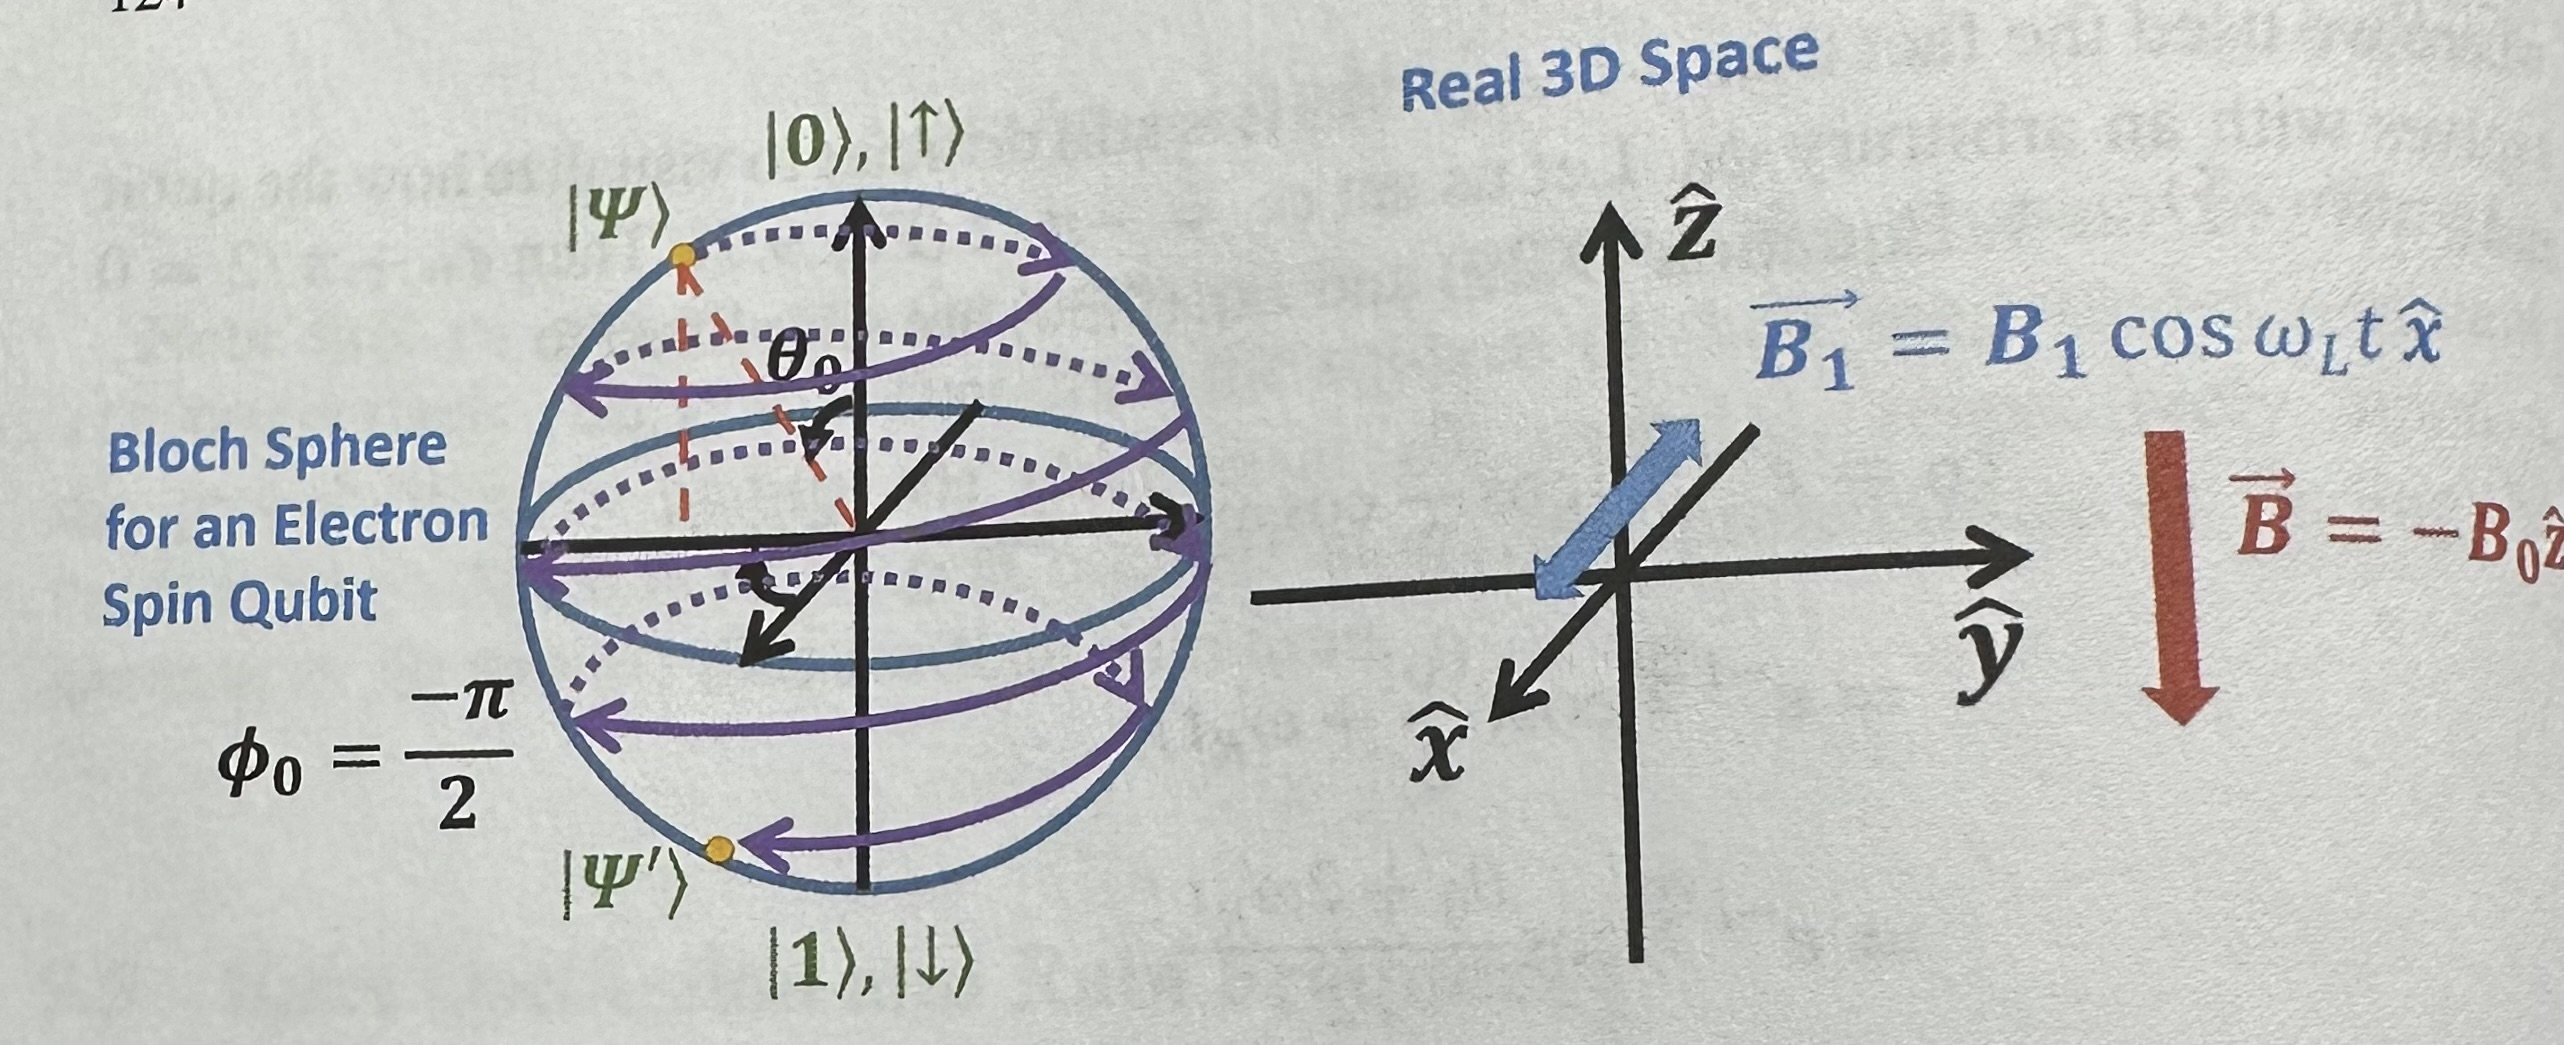
\includegraphics[scale=0.5]{fig. 9.2.jpeg}\\
\textbf{Fig. 9.2} Rabi oscillation at spin resonance when the horizontal field is oscillating at Larmor frequency ($\omega_1=\omega_L$).
The initial state $\ket{\Psi}$ has an initial azimuthal angle $\phi_0=\pi/2$. The left shows how the state moves on the Bloch sphere due to 
Larmor precession and Rabi oscillation. The right shows the setup of the experiment\\

Again we have already set $\phi_0=\pi/2$ to achieve this result. Like Eq. (8.10), this equation tells us that the zimuthal angle,
i.e., $\phi_0-\omega_L t$, reduces at a rate of $\omega_L$. This is the Larmor precession due to the vertical constant magnetic field.
At the same time, the polar angle also changes as $\theta_0+\omega_Rt$ which means it changes at a rate of the Rabi frequency, $\omega_R$
(Fig. 9.2).\\\\
\textbf{Example 9.2} It is instructive to understand Rabi oscillation and Rabi frequency by
examing the change of probability of measuring $\ket{0}$ and $\ket{1}$ as a function of time.

Let us still consider the case when $\phi_0=\pi/2$. We will also set $\theta_0=0$ which
means the initial state is the "north pole" of the Bloch sphere. Based on Eq. (9.34), the state
as a function of time becomes,
\begin{align*}\label{eq 9.35}
    \ket{\Psi}&=e^{-i\frac{\phi_0-\omega_Lt}{2}}\cos\frac{0+\omega_Rt}{2}\ket{0}+
    e^{i\frac{\phi_0-\omega_Lt}{2}}\sin\frac{0+\omega_Rt}{2}\ket{1},\\
    &=e^{-i\frac{\phi_0-\omega_Lt}{2}}\cos\frac{\omega_Rt}{2}\ket{0}+
    e^{i\frac{\phi_0-\omega_Lt}{2}}\sin\frac{\omega_Rt}{2}\ket{1}.\tag{9.35}
\end{align*}

The probability of finding the state at $\ket{0}$, \textit{$P_0$}, is thus $|e^{-i\frac{\phi_0-\omega_Lt}{2}}\cos\frac{\omega_Rt}{2}|^2$
because it it the square of the magnitude of the coefficient of $\ket{0}$. Therefore, $P_0=\cos^2\frac{\omega_Rt}{2}$
because the exponential term has a unity length. Similarly, the probability of finding the state at $\ket{1}, P_1,$ is $\sin^2\frac{\omega_Rt}{2}$.

Since both $P_0$ and $P_1$ are the square of a sinusoidal function, they have a period of $\pi$ and have
values between 0 and 1, which is expected as they are probabilities. Therefore, they repeat
when $\frac{\omega_Rt}{2}=\pi$. In other words, they have a period of $T=\frac{2\pi}{\omega_R}$,
Figure 9.3 plots $P_0$ and $P_1$ as a function of time when $\omega_R=2\pi\times50kHz$. It has a period of 
$T=\frac{2\pi}{2\pi\times50kHz}=20\mu s$.\hfill $\blacksquare$


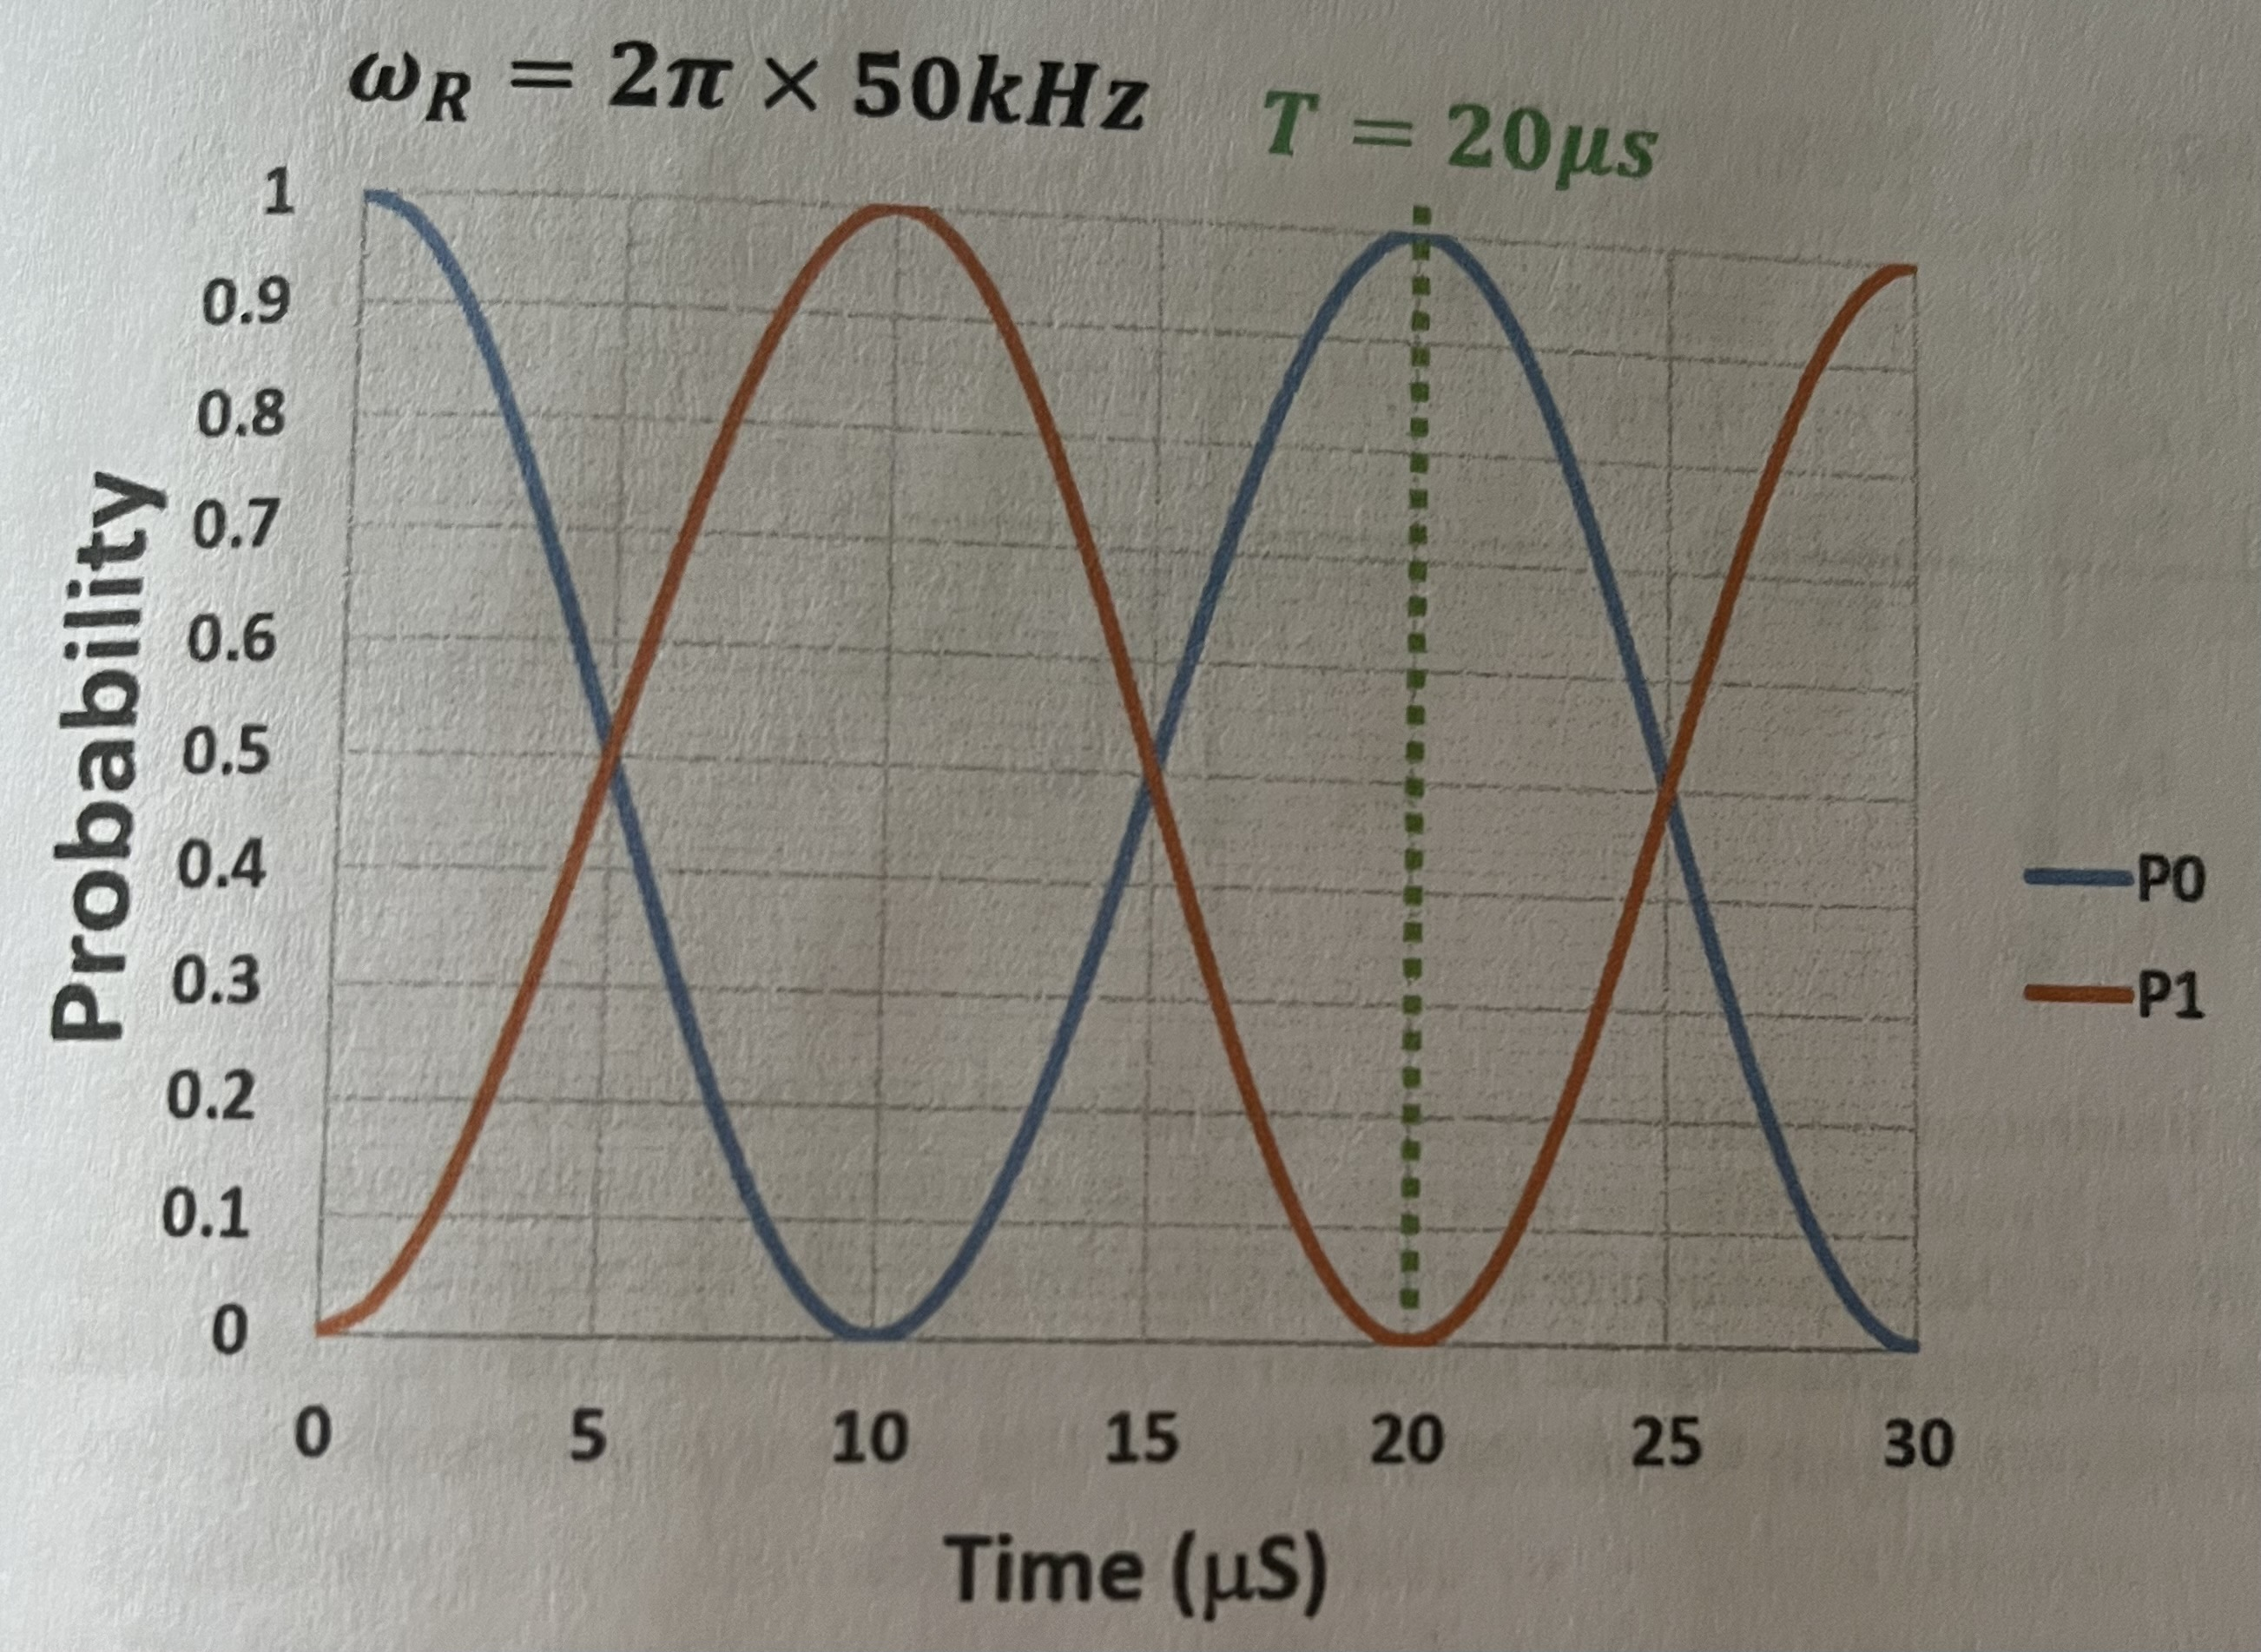
\includegraphics[scale=0.45]{Fig.9.3.jpeg}\\
\textbf{Fig 9.3} Plots of $P_0$ and $P_1$ as a function of time when $\omega_R=2\pi\times50kHz$\\\\\\
\textbf{\large 9.6 Intuitive View of Spin Resonance and Rotating Wave Approximation}\\\\
Let us know gain more insight into the physics of the horizontal oscillating field. Since it is at spin
resonance, the field is oscillating at Larmor frequencey. The osciallation field is copied from Eq. (\ref{eq 9.5}) with
$\omega_1=\omega_L$ as,
\begin{align*}\label{eq 9.36}
    \vec{B_1}&=B_1\cos(\omega_1t)\hat{x},\\
    &=\frac{B_1}{2}(\cos(\omega_1t)\hat{x}+\sin(\omega_1t)\hat{y}+\cos(\omega_1t)\hat{x}-\sin(\omega_1t)\hat{y},\\
    &=\vec{B_{1+}}+\vec{B_{1-}}, \tag{9.36}
\end{align*}
where in line 2, the two sine term can be canceled to restore line 1. In line 2, we made the 
following definitions:
\begin{equation}\label{eq 9.37}
    \vec{B_{1+}}=\frac{B_1}{2}(\cos(\omega_1t)\hat{x}+\sin(\omega_1t)\hat{y}).\tag{9.37}
\end{equation}
\begin{equation}\label{eq 9.38}
    \vec{B_{1-}}=\frac{B_1}{2}(\cos(\omega_1t)\hat{x}-\sin(\omega_1t)\hat{y}).\tag{9.38}
\end{equation}
Therefore, the linearly oscillating field in the $\hat{x}$ direction is decomposed into the
sum of one clockwise, $\vec{B_{1-}}$, and one counterclockwise, $\vec{B_{1+}}$, rotating field with
half of the original strenght ($B_1/2$) at Larmor frequency (middle of Fig. 9.4).

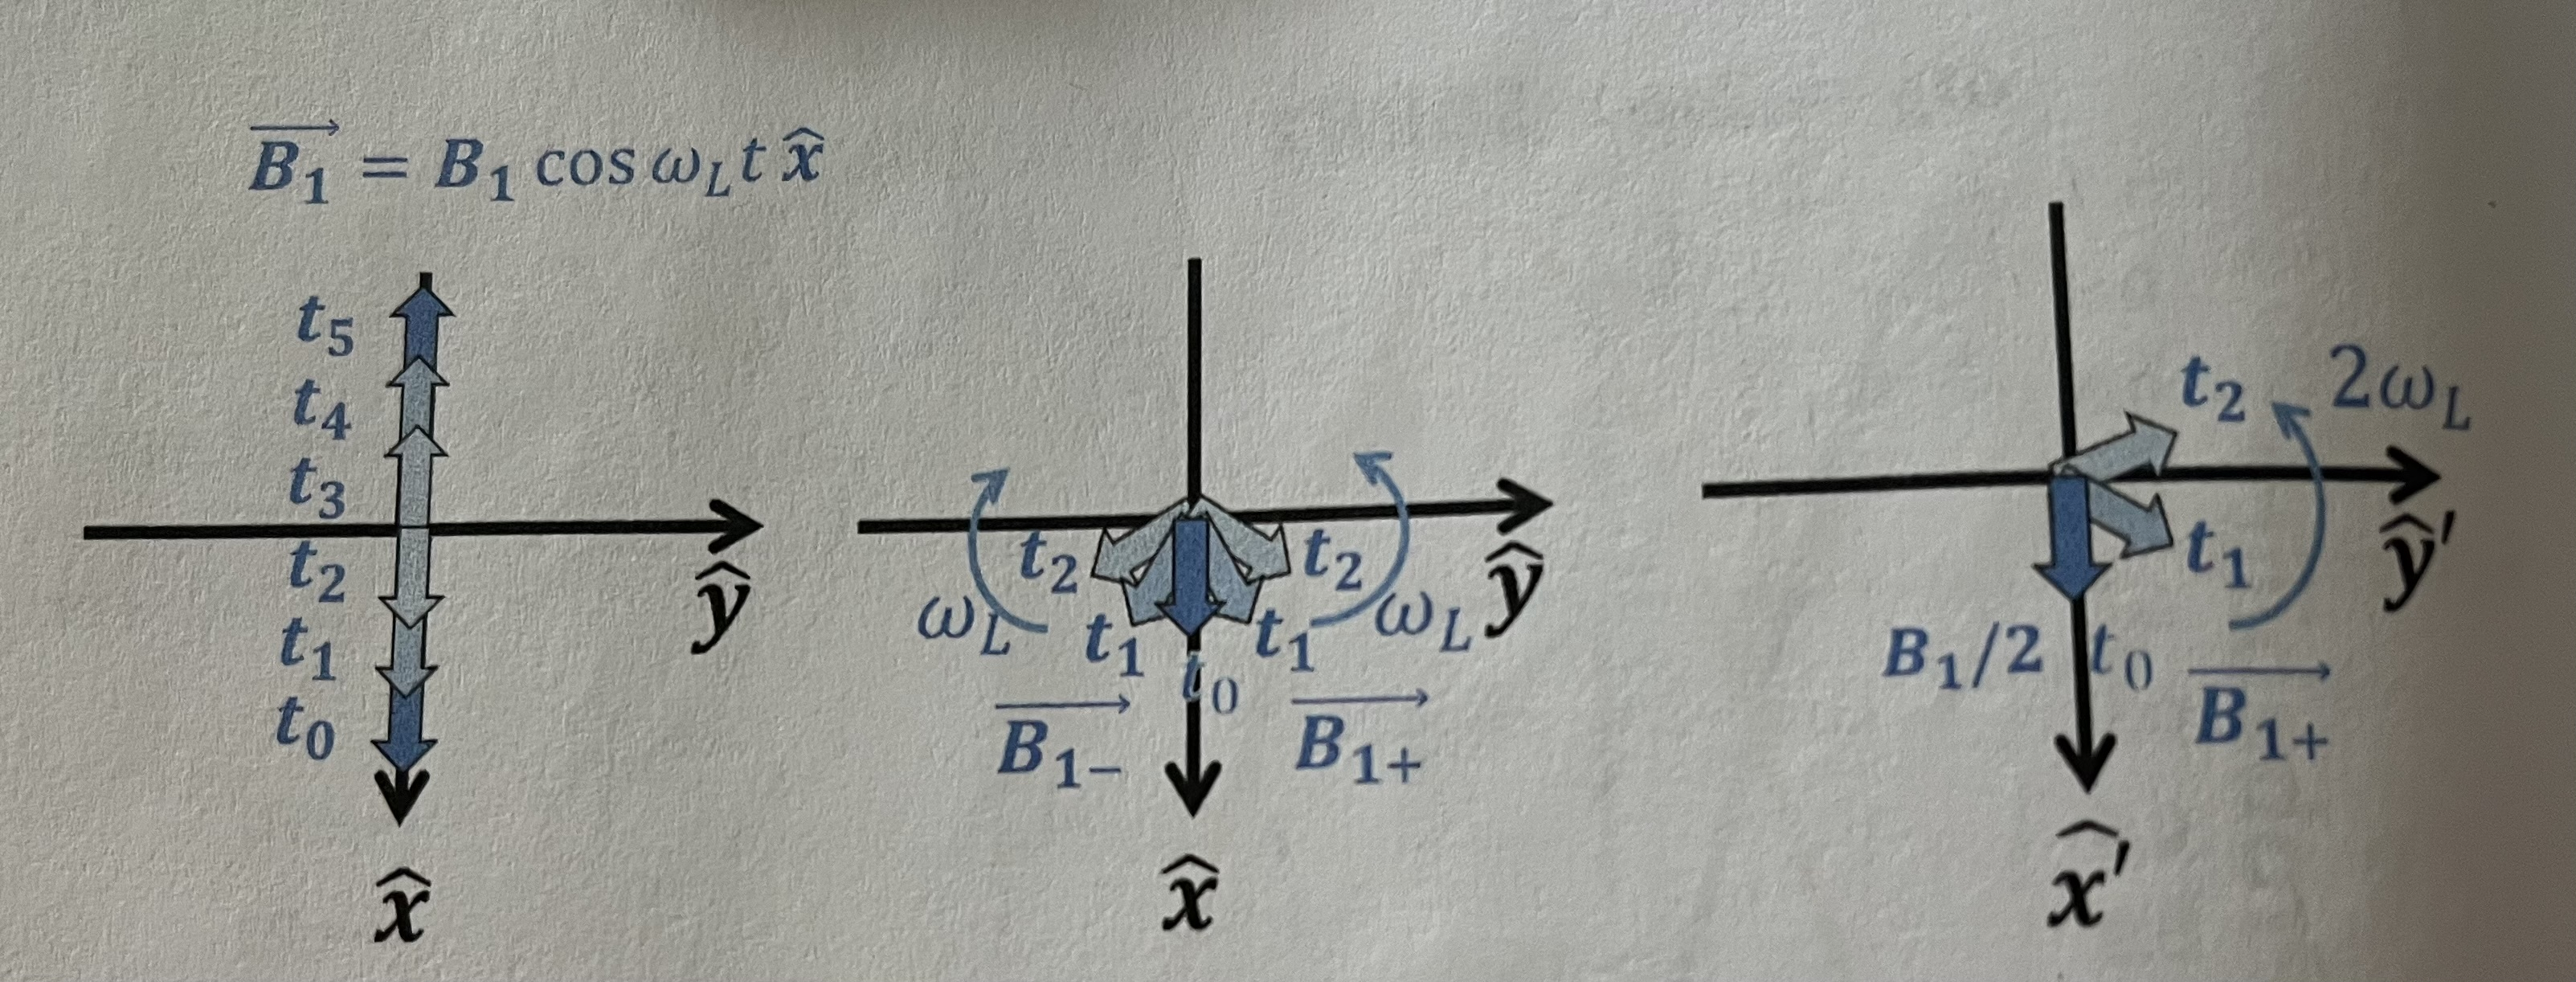
\includegraphics[scale=0.4]{Fig.9.4.jpeg}\\
\textbf{Fig. 9.4} Illustration of rotation wave approximation at spin resonance when $\omega_L=\omega_1$.
Left: The change of the linearly oscillating magnetic field as a function of time with $t_0<t_1<t_2<t_3<t_4<t_5$.
Middle: Decompostition of the linearly oscillating magnetic field into two rotating fields at 
$t_0, t_1,$ and $t_2$. Right: Tranform the system to a rotating frame of Larmor precession where 
$\vec{B_{1-}}$ is followed and fixed. $\vec{B_{1+}}$ is then appeared to be rotating at an angular frequency of 2$\omega_L$ \\\\

Now, if we follow $\vec{B_{1-}}$, then $\vec{B_{1-}}$ is not moving. This is a new frame ($\hat{x}^\prime-\hat{y}^\prime$ at the right of Fig. 9.4)
and we call it the \textbf{rotating frame} in contrast to the laboratory frame ($\hat{x})-\hat{y}$ at the middle of Fig. 9.4) where
we usually stay. This is similar to the situation that if we are in an amusement park and stay on
the ground (laboratory frame), we see the merry-go-round rotating. If we jump on the merry-go-round,
the merry-go-round is no longer rotating to us and we are in the rotating frame. With
this, we feel a constant magnetic field, $B_1/2$, pointing in the $\hat{x}^\prime$ direction
due to $\vec{B_{1-}}$. Moreover, we also feel that $\vec{B_{1+}}$ is rotating at a rate of $2\omega_L$ away
from us. If for the action we are interested in, the rotation of $\vec{B_{1+}}$. is rotating at a rate of 
$2\omega_L$ away from us. If for the action we are interested in, the rotation of $\vec{B_{1+}}$ is fast,
then it might have rotated many cycles before we complete any meaningful action. As a result, we will not feel
its effect. This is because $\vec{B_{1+}}$ has swept throught all direction
on the plane. Imagine that you stand still and someone pushes you from all direction within a
short time; overall, there is no net effect. This is the \textbf{rotating wave approximation}
in Eq. (\ref{eq 9.22}) where the effect of $e^-i2\omega_Lt$ was ignored.

In the rotating frame, we only have a constant field, $B_1/2$, in the $\hat{x}^\prime$ direction.
This is just like the case of a constant external magnetic field and we expect that there will be Larmor
precession. But this time it will precess about the $\hat{x}^\prime$ axis.
Based on Eq. (8.11), it will precess at an angular frequency of $\frac{e}{m}B_1/2$ because the
constant magnetic field has a value of $B_1/2$ instead of $B_0$. \textbf{And this is the same
as the Rabi frequency we derived in Eq. (\ref{eq 9.32})!} Therefore, Rabi oscillation in the
rotating frame is just the Larmor precession about $\hat{x}^\prime$.

When we are in the rotating frame, we can ignore the vertical magnetic field. We can understand
this from another point of view. Since $B_1\ll B_0$, we can assume the Larmor precession due to the 
vertical field is not affexted and the effect of the horizontal rotating field can be simply added on
top of the Larmor precession. So if we are already working in the rotating frame. $\boldsymbol{H_0}$ can be
ignored because the rotating frame goes at the same angular velocity as the precession due to the
vertical magnetic field.

I will leave this as an exercise. What is the Larmor precession direction in the rotating frame due to 
$B_1/r\hat{x}^\prime$? Is it consistent with the direction shown in Fig. 9.2?

Lastly, ley us dicuss when RWA is valid. As mentionedm it is valid if the action
we are interested in has a much longer time than $1/(2\omega_L)$. For example, if we are implementing a quantum
gate to rotate qubits about $\hat{x}$-axis using Rabi oscillation,
we want $1/\omega_R\gg 1/(2\omega_L)$. This is usually true because $1/\omega_R$ is in the 
$\mu_s$ range (Fig. 9.3) and $1/(2\omega_L)$ is much smaller.\\\\\\
\textbf{\large 9.7 Summary}\\\\
There are a lot of equations in this chapter. However, it is worthwhile to 
follow to understand the details. because they reinforce our understanding of some of
the critical concepts. We show that by applying an oscillating magnetic field in
the $\hat{x}$ direction in addition to the constant megnetic field in $-\hat{z}$, it is 
possible to move a state from the upper hemisphere of the Bloch sphere to the lower hemisphere.
To solve the problem, we introduce the concept of the angular momentum operator.
The oscillating magnetic field is usually much smaller thant the constant magnetic field.
This allows us to use perturbation theory to simplify the problem. We further apply
the oscillating field at the same frequency as Larmore precession, resulting in spin resonance.
Then we apply rotating wave approximation by ignoring the high frequency part to arrive
at the final solution to understand Rabi oscillation better. It is also very instructive to see
the problem in the rotating frame to realize that Rabi oscillation in the laboratory frame is just
the Larmor precession about the $\hat{x}^\prime$-axis in the rotating frame.\\\\\\
\textbf{\large Problems}\\\\
\textbf{9.1 Spin Angular Momentum Operator}\\
Show that
\begin{equation}\label{eq 9.39}
    \braket{1|\vec{S}|1}=-\frac{\hbar}{2}\hat{z},\tag{9.39}
\end{equation}
\begin{equation}\label{eq 9.40}
    \braket{+|\vec{S}|+}=\frac{\hbar}{2}\hat{x}.\tag{9.40}
\end{equation}
\textbf{9.2 Hamiltonian Elecments}\\
Redo Eqs. (\ref{eq 9.15}) and (\ref{eq 9.16}) using $\boldsymbol{H_0}=-\frac{\hbar\omega_L}{2}\boldsymbol{\sigma_z}$.\\\\
\textbf{9.3 Solving Schr\"{o}dinger Equation}\\
Derive Eq. (\ref{eq 9.21}) by following the approach for Eq. (\ref{eq 9.20}).\\\\
\textbf{9.4 Rabi Oscillation 1}\\
If $B_1=0.01 T$, compare the Rabi oscialltion period to the gate time in Problem 8.2\\\\
\textbf{9.5 Rabi Oscillation 2}\\
Discuss if the Larmor precession in the rotating frame has the same direction as Rabi oscillation in the laboratory frame.\\\\\\
\textbf{\large References}\\\\
1. Hiu-Yung Wong. \textit{Introduction to Quantum Computing}. Springer, 2024.\\
2. David J. Griffiths. \textit{Introduction to Quantum Mechanics}. Pearson College Div, 1994.\\
3. Erwin Kreyszig. \textit{Advanced Engineering Mathematics}. John Wiley \& Sons; 9th Edition, International Edition. 2006

\end{document}